\documentclass[12pt]{article}

% Preamble!!
\usepackage{titlesec}
\titlelabel{\thetitle.\quad}
\usepackage{xcolor}
\usepackage{adjustbox}
\usepackage{amsmath}
\usepackage{amsthm}
\usepackage{amsfonts}
\usepackage{amssymb}
\usepackage{graphicx}
\usepackage{setspace}
\usepackage{longtable}
\usepackage{lscape}
\usepackage{indentfirst}
\usepackage[labelsep=period,justification=justified,singlelinecheck=false,font = footnotesize, labelfont=bf]{caption}
\usepackage{booktabs}
\usepackage{tabularx,ragged2e}
\usepackage{natbib}
\usepackage{rotating}
\usepackage{placeins}
\usepackage[bookmarks=true,bookmarksnumbered=true, hypertexnames=false,breaklinks=true,citebordercolor={1 1 1},pdfborder={1 1 1},
pdfauthor={},pdftitle={},pdfdisplaydoctitle=true]{hyperref}
\usepackage{array}

\RequirePackage{etoolbox}
\pdfoutput=1

\usepackage{epstopdf}
\usepackage{wrapfig}
\usepackage{subfigure}
\usepackage{float}
\usepackage[justification=centering]{caption}

\let\ORGsidewaysfigure\sidewaysfigure
\let\ORGendsidewaysfigure\endsidewaysfigure
\renewenvironment{sidewaysfigure}
  {\ORGsidewaysfigure\vspace*{.5\textwidth}\begin{minipage}{\textheight}\centering}
  {\end{minipage}\ORGendsidewaysfigure}

\usepackage{epstopdf}
\DeclareGraphicsRule{.tif}{png}{.png}{`convert #1 `dirname #1`/`basename #1 .tif`.png}


\newcommand\mat[1]{\mathcal{#1}}
\newcommand\norm[1]{\left\lVert#1\right\rVert}
\renewcommand{\familydefault}{\rmdefault}



\newcommand{\E}{\mbox{E}}
\newcommand{\X}{\mbox{X}}
\newcommand{\mX}{\mathbf{X}}

\newcommand{\Y}{\mbox{Y}}

\newcommand{\N}{\mbox{N}}
\newcommand{\I}{\mbox{I}}
\newcommand{\muxy}{\frac{n}{n+m}\mu_y + \frac{m}{n+m}\mu_x}
\newcommand{\J}{\mbox{J}}
\newcommand{\Om}{\boldsymbol{\Omega}}
\newcommand{\Lim}[1]{\raisebox{0.5ex}{\scalebox{0.8}{$\displaystyle \lim_{#1}\;$}}}
\newtheorem*{remark}{Remark}
\newcommand{\appropto}{\mathrel{\vcenter{
  \offinterlineskip\halign{\hfil$##$\cr
    \propto\cr\noalign{\kern2pt}\sim\cr\noalign{\kern-2pt}}}}}
\newcommand\independent{\protect\mathpalette{\protect\independenT}{\perp}}
\def\independenT#1#2{\mathrel{\rlap{$#1#2$}\mkern2mu{#1#2}}}


\newcolumntype{Y}{>{\centering\arraybackslash}X}
\providecommand{\U}[1]{\protect\rule{.1in}{.1in}}
\providecommand{\U}[1]{\protect\rule{.1in}{.1in}}
\providecommand{\U}[1]{\protect\rule{.1in}{.1in}}
\providecommand{\U}[1]{\protect\rule{.1in}{.1in}}
\setlength {\topmargin}{-0.11in}\setlength {\headheight}{0in}
\setlength
{\headsep}{0in}\setlength{\textwidth}{6.65in}
\setlength
{\oddsidemargin}{-0.054in}\setlength {\textheight}{8.995in}
\setlength
{\marginparsep}{0in}\setlength {\marginparwidth}{0in}
\captionsetup[table]{labelsep=colon}

\renewcommand{\arraystretch}{0.7}


\theoremstyle{plain}
\newtheorem{thm}{Theorem}[section]


% Beginning the document!!


\begin{document}

\title{Financial Literacy and Economic Outcomes}
\author{
\textbf{David Puelz}\thanks{The University of Chicago. Email: david.puelz@chicagobooth.edu} \\ \and \textbf{Robert Puelz}\thanks{Southern Methodist University. Email: rpuelz@mail.cox.smu.edu}
}
\date{}
\maketitle\thispagestyle{empty}


\begin{center}

\vspace{0.3in}

\begin{abstract}
We explore the relationship between financial literacy and self-reported economic outcomes using survey data from the United States.  Our dataset includes several measured covariates of the survey individuals, and we use a new econometric technique developed by \cite{hahn2018regularization} to control for the appropriate confounders.  We report treatment effect estimates describing the relationship between literacy and economic outcomes.
\end{abstract}

\vspace{1.5in}
\end{center}

\textbf{Keywords:} Financial Literacy, Economic Outcomes, Treatment Effect Estimation

\setcounter{page}{0}\thispagestyle{empty}\baselineskip18.99pt\newpage 
\setstretch{1}

\clearpage

\pagestyle{plain}

\section{Introduction}
Is financial literacy associated with a household achieving more financial happiness?  There is natural presumption that basic literacy is good and gradations of increasing financial literacy are better. Interest and education in financial literacy in the United States has become widespread and institutionalized by the Federal Reserve that has taken an active role in creating financial information for individuals.\footnote{As an example of financial education sources the U.S Treasury department has compiled a list. See \href{https://www.treasury.gov/resource-center/financial-education/Documents/OFE-CFAP-Resources.pdf}{https://www.treasury.gov/resource-center/financial-education/Documents/OFE-CFAP-Resources.pdf}, and the Chicago FED lists educational offerings of banks in the system. See \href{https://www.chicagofed.org/region/community-development/cedric/federal-reserve-financial-education-initiatives}{https://www.chicagofed.org/region/community-development/cedric/federal-reserve-financial-education-initiatives}}.  Books on personal finance, investing, and wealth creation have become as ubiquitous as books on health and weight loss.

One objective of investing in financial knowledge is clear:  a household will have a better chance at optimizing their living standard if they are financially adept.  Specialized knowledge appears to be important and just being educated does not enable competence about personal finance.  \cite{mitchell2015financial} find that increased education and financial literacy are positively correlated, yet they find less than 50\% of college-educated students can successfully answer three key financial literacy questions and less than 64\% of students with a post-graduate education can answer all three questions correctly.  Perhaps ``interventionist'' activity is needed.  \cite{elylecture} has argued that important questions about financial regulations surrounding household finance are ripe for the attention of economists because there is not much known about how consumer financial regulatory costs would be offset by its benefits.

There is a large body of more recent research summarized by \cite{hastings2013financial} and \cite{lusardi2014economic} that trace many of the key questions around a more financially literate populace to education choices, the timing of education delivery during an individual’s life-cycle, public policy prescriptions, and regulatory intervention.  What is less well understood is the link that can address the question whether being personally financially literate matters to economic outcomes? Anecdotally, it is nearly impossible to argue that some personal financial knowledge is unimportant to a household's economic outcomes, however individuals rely on the specialist knowledge of others to diagnose illnesses, construct legal documents, even to prepare a good meal.  We heed the call of others to strengthen our understanding of the connection between financial competence and financial outcomes.\footnote{As noted by \cite{lusardi2014economic}, p. 34, ``Though it is challenging to establish a causal link between financial literacy and economic behavior, both instrumental variables and experimental approaches suggest that financial literacy plays a role in influencing financial decision making, and the causality goes from knowledge to behavior.''  
Two noteworthy contributions along this path are \cite{calvet2007down} and \cite{agarwal2009age}} 

We begin by isolating economic outcomes from behaviors for the data generated from FINRA's complete 2015 National Financial Capability Survey study.  We identify five survey questions that reveal actual respondent economic outcomes.  Further, we categorize a number of good and and bad financial practice behaviors and include numerous other respondent and household factors that are plausibly related to economic outcomes, including the financial literacy treatment.   In this study we are interested in two questions:  

\begin{enumerate}
\item Is there a systematic relationship between individuals who experiences a negative financial outcome and their financial literacy?
\item Is financial literacy separable?  For instance, is being financially literate on one topic sufficient for positive economic outcomes, and conversely is limited financial literacy on one topic sufficient for a negative economic outcome? 
\end{enumerate}

To answer these questions we recognize the potential for bias in any estimations because the literacy treatment variable is correlated with a dependent variable and a set of covariates.  Moreover, the dimensions of the final sample from the NCFS study are characterized by a large number of covariates and a relatively limited observations count making more traditional estimation approaches problematic.\footnote{Indeed, most empirical questions surrounding financial literacy are characterized by these problems.}  To resolve the statistical problem we apply the work of \cite{hahn2018regularization} who call on recent research in treatment effect estimation and machine learning.  \cite{hahn2018regularization} describe a data-driven approach to identify confounders and mitigate treatment effect estimation bias.  To analyze the relationship between literacy and economic outcomes, only \textit{one model} with all available covariates needs to be specified, and the data will select the meaningful ones.\footnote{  They propose jointly modeling the treatment and response $Y,Z \mid \text{X}$ by first modeling the treatment variable as a function of covariates $Z \mid \text{X}$, and then modeling the response $Y \mid Z,\text{X}$.  The first likelihood provides information on the propensity of being treated as a function of covariates, and the second utilizes this information to mitigate endogeneity when estimating the partial effect of $Z$ on $Y$. Importantly, their procedure provides a way to ``shrink-away'' irrelevant covariates using Bayesian shrinkage priors.}

 
We find .....

\section{Literature Review}
It is well-documented that U.S. citizens have low levels of financial knowledge and make financial ``mistakes.'' \cite{calvet2009measuring} created an index of financial sophistication from mistakes related to under diversification, risky share turnover and the disposition effect and find that less sophistication is related to individuals with less wealth, smaller family size, less education  and less financial experience.\footnote{\cite{odean1998investors} defined the disposition effect as the tendency for investors who hold losers to hold them too long, and investors who own winners to have sold them too quickly. }  \cite{choi2011100} found that more than a third of employees do not take advantage of an employer match to a 401(k) plan when it is clearly to their benefit to do so.\footnote{\cite{choi2011100} sample included employees who were older than 59.5 who were unconstrained by withdrawal penalties: they could have simply withdrew employer contributions but chose not to take advantage of it.   Even among a subsequent experiment, the researchers find conclude that low financial literacy and poor choice about a matching contribution are positively related.}    \cite{keys2016failure} found that 20\% of households do not refinance their mortgage even when it is to their benefit.  Recently, \cite{systematicmistakes} found the individuals who opt for points in their mortgages, a poor financial choice in their analysis, are less responsive to interest rate changes and preferred refinancing behavior.

The literature suggests that investments in financial education may not be helpful in solving the problem of poor financial choices, contrary to intuition.   \cite{willis2008against} confronts the idea that financial education is inherently a good idea by taking the view that a ``financial regulation-through-education policy model'' imposes costs on those aspiring to be financial literate that are significantly higher than the benefits from the financial literacy gained.\footnote{See \cite{willis2008against}, p. 204.  Willis interprets policymakers’ promotion of financial literacy as an ineffective substitute for financial regulation that places too high a burden on non-expert consumers.}   Policymakers who promote financial literacy as important intend, at least partly, to have the individual bear responsibility for the management of his or her financial future.  Indeed, \cite{willis2011financial} asserts that financial regulation replaced by financial education is a ``fundamental fallacy.''\footnote{See \cite{willis2011financial} p. 429.}   The individual would always be chasing the details of new product innovation and once the consumer shortens their information disadvantage, Willis argues that the industry would ``outmaneuver'' them.  \cite{willis2011financial} notes that empirical work to date is replete with evidence that ``biases, heuristics, and other nonrational influences'' circumvent good financial decision-making.   \cite{lusardi2017optimal} develop a model that includes the prospect of financial knowledge investment, and illustrate conditions under which less investment is preferred.    The implication is that if financially literate consumers do not make better financial decisions, then personal investments in financial knowledge are best not incurred.

If education would not be helpful, then how do consumers plan well for their financial futures?  \cite{calcagno2015financial} offer a different perspective.  They start with a premise that those who are less financially literate may benefit from more personal finance advice or derive more value from a financial adviser.  They construct a theoretical model that considers an adviser who has the ability to sell investments and is compensated by a proportional commission linked to the size of the investment. The adviser's customer may be asymmetrically informed about the attributes of candidate investments.  Considering incentives, penalties and information costs, their model predicts that those who are better informed are more likely to invest in risky assets and utilize a financial adviser.  Indeed, the authors use bank survey data from Italy to find empirically that utilization of financial advisers is higher among those who are already financially literate, and that financial literacy is positively related to the probability of investing in risky assets.\footnote{\cite{almenberg2015gender} link financial literacy and investing in the stock market with the intent to explore how investing varies between men and women when financial literacy is controlled.  The authors measure financial literacy by identifying basic and advanced financial skills.  While the authors find that men have higher probabilities of investing in the stock market, controlling for financial literacy skills reduces the probability differences between men and women substantially, and makes a ``gender gap,'' inconsequential.}   In a different yet relevant study, \cite{advisorsBandB2016} used 2012 NFCS survey data and an instrumental variables approach to mostly corroborate Calcagno and Monticone's empirical results.  Balasubramnian and Brisker defined advisers by their role with a survey participant (e.g., Investment adviser, Debt Counselor, Tax adviser and so forth) if such a relationship existed at all.\footnote{53.4\% of Balasubramnian and Brisker's sample used one of the defined advisers.}   The researchers found  a positive relationship between working with an investment financial adviser and financial literacy, although they found a negative relationship for those who worked with a debt consolidation adviser. 

The literature to date supports the conclusions that households error in their decision-making, more highly educated individuals are not inclined to be better at making financial decisions, and that investments in financial literacy have low payoffs.   More sophisticated individuals may be more inclined to hire financial advisers, but is that a good idea, and do individuals of any sophistication level know there are differences in how advisers are paid and the incentives that drive their recommendations?   There are good reasons for consideration of a third-party who can force guidance on consumers in the spirit of the arguments presented by \cite{elylecture}.   The promotion for more financial literacy, however delivered, suggests that not enough is yet known about whether financial literacy can create good economic outcomes.  We supplement the mistakes literature by taking a different tack.  That is, among those individuals who are most financially literate, do they have financial outcomes that we can describe as good?

\section{The Study}
The NFCS survey provides reasonable proxies of economic outcomes based on answers given by respondents to survey questions sprinkled through out the questionnaire.\footnote{Generally, the economic outcome for a household at any point in time is its economic net worth; that is, assets including household human capital less debt.}    We identified five questions used in the 2015 National Financial Capability Study, that are representations by respondents about their current financial circumstance.\footnote{Studies were conducted in 2009, 2012 and 2015.  See \href{http://www.usfinancialcapability.org}{http://www.usfinancialcapability.org}.}  They are the following:

\begin{enumerate}
\item ``Overall, thinking of your assets, debts and savings, how satisfied are you with your current personal financial condition?'' %This is J1 in data
\item ``In the last 12 months, have you [or your spouse/partner] taken a
hardship withdrawal from your retirement account(s)?'' %\textcolor{red}{[This is C10\_2012 in data, not sure we can focus on this because I don't believe this variable exists for 2015...]}
\item ``Are you concerned that you might not be able to pay off your student loans?'' % This is G22_2015 in the data
\item ``In a typical month, how difficult is it for you to cover your expenses and pay all your bills?'' % This is J4
\item ``How strongly do you agree or disagree with the following statement? - I have too much debt right now'' % This is G23
\end{enumerate}

Using respondent responses to each of these five questions we call on  \cite{wittkowski2004combining} who provide.........


\subsection{The Data and Initial Analysis} \label{initial}
We start with the full data set from the 2015 NFCS study made available to us by FINRA.  There are 27,564 observations and 149 variables.  In our approach, we require complete data across 117 covariates and dummy variables which limits the total number of observations to 997.  

\subsubsection{Dependent Variable}

Our dependent variable of interest is an economic outcome index that is created from the responses to the economic outcome questions which are summarized in Tables \ref{tab:dependents} and \ref{tab:dependents2}.  Questions 1,4, and 5 are measured on integer scales from 1 to 10, 1 to 3, and 1 to 7, respectively.  The mean, minimum, and maximum values  are displayed in \ref{tab:dependents}.  Questions 2 and 3 are binary variables, so we display their summary statistics in Table \ref{tab:dependents2}.

\begin{table}[H]
\centering
\caption{Responses to questions used to construct the economic outcome (dependent) variable: Summary statistics for quantitative variables across the NFCS sample of 997 observations.}
\renewcommand{\arraystretch}{1}
\begin{tabular} {|c|c|c|c|}

\hline
\ & \textbf{Q1} & \textbf{Q4} & \textbf{Q5} \\ [0.5ex] 
 \hline\hline
 mean & 6.7 & 2.3 & 5.1 \\
  \hline
 min & 1 & 1 & 1 \\
  \hline
 max & 10 & 3 & 7\\
  \hline
 s.d. & 2.5 & 0.7 & 1.8\\
 \hline
\end{tabular}
\label{tab:dependents}
\end{table}

\begin{table}[H]
\centering
\caption{Responses to questions used to construct the economic outcome (dependent) variable: Summary statistics for binary variables across the NFCS sample of 997 observations.}
\renewcommand{\arraystretch}{1}
\begin{tabular} {|c|c|c|}

 \hline
\ & \textbf{Q2} & \textbf{{Q3}}\\ [0.5ex] 
 \hline \hline
\% No & 72\% & 58\% \\
 \hline
\% Yes & 28\% & 42\%  \\
 \hline
\end{tabular}
\label{tab:dependents2}
\end{table}


These five questions comprise our measures of economic outcomes for individuals in the sample.  In Section \ref{statmethods}, we discuss how we combine this information from multiple outcomes into a single, meaningful measure. 

\subsubsection{The Financial Literacy Variable}

The strength of the connection between economic outcomes and financial literacy is tested with a measure for financial literacy that is the total number of correct answers to six financial literacy questions included in the 2015 survey and reported in Table \ref{tab:literacy}.\footnote{The interest rate, inflation and risk questions were designed by Olivia Mitchell and Annamaria Lusardi.  See \cite{lusardi2014economic}.  According to the \href{http://www.usfinancialcapability.org/downloads/NFCS\_2015\_Report\_Natl\_Findings.pdf}{2015 NFCS national report}, the Rule of 72 question was added as an additional interest rate question to `` to test the concept of interest compounding in the context of debt.''} Figure \ref{indvar} is a column chart that summarizes the percentage of correct answers for each of the six financial literacy questions across the sample.  Relatively higher proportions of respondents were successful at answering correctly the savings account growth question (``Interest rate'') and the mortgage payment and mortgage interest paid (``Mortgage'') question.  More than 60\% of respondents did not understand the relationship between a bond's value and market interest rates (``Bond price''), and about half of the respondents proved adept at questions related to inflation, the rule of 72 and risk. The six questions taken together across the final sample showed a  mean number of correct answers of \textbf{3.86}.  

%The tables need to have formatting cleaned up but the content is on par
\begin{table}[H]
\centering
\caption{Financial Literacy Questions}
\renewcommand{\arraystretch}{1}
\begin{tabular} {|c|p{13.3cm}|}

 \hline
\textbf{Concept addressed} & \textbf{Question}\\ [0.5 ex] 
 \hline \hline


Interest rate & Suppose you had \$100 in a savings account and the interest rate was 2\%
per year. After 5 years, how much do you think you would have in the
account if you left the money to grow?\\
 \hline
Inflation &	Imagine that the interest rate on your savings account was 1\% per year and inflation was 2\% per year. After 1 year, how much would you be able
to buy with the money in this account?\\
\hline
Bond price &	If interest rates rise, what will typically happen to bond prices?\\
\hline
Rule of 72 &	Suppose you owe \$1,000 on a loan and the interest rate you are charged is 20\% per year compounded annually. If you didn’t pay anything off, at this interest rate, how many years would it take for the amount you owe to double\\
\hline
Mortgage &	15-year mortgage typically requires higher monthly payments than a
30-year mortgage, but the total interest paid over the life of the loan
will be less.
Measurement Level: Nominal\\
\hline
Risk &	Buying a single company's stock usually provides a safer return than a
stock mutual fund.\\
\hline
\end{tabular}
\label{tab:literacy}
\end{table}



\begin{figure}[H]
\centering
\caption{Proportion of correct answers for each of the six financial literacy questions displayed in Table \ref{tab:literacy}.}
	\centerline{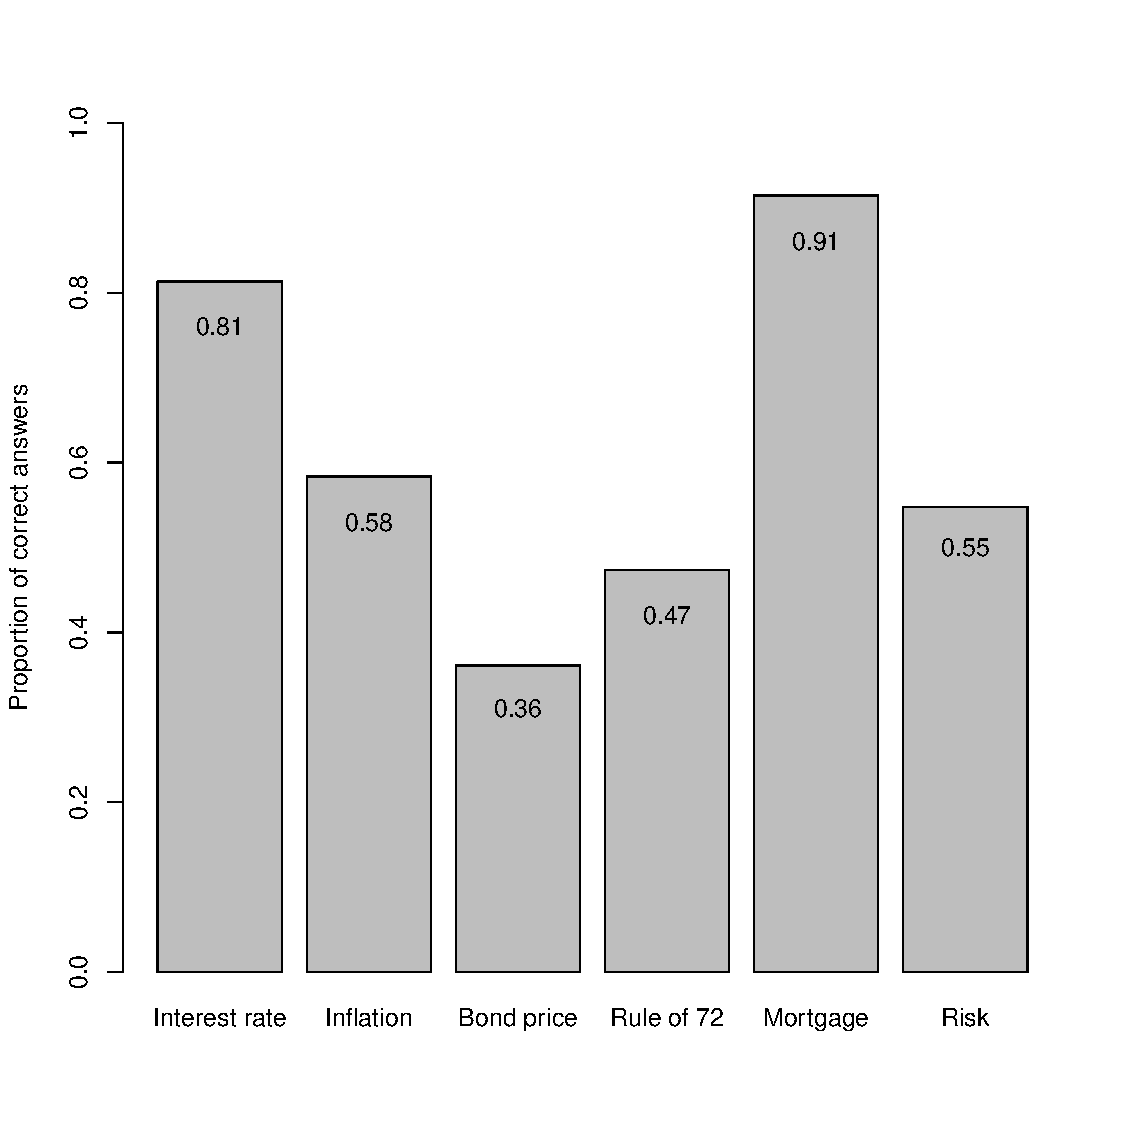
\includegraphics[scale=.6]{barplot_ind.pdf}}\label{indvar}
\end{figure}


\subsubsection{Additional Control Variables}

Generally, descriptive statistics of the NFCS data have been reported by many researchers including the NFCS itself, and we follow accordingly for the data used in this paper.\footnote{See \href{http://www.usfinancialcapability.org/results.php?region=US}{http://www.usfinancialcapability.org/results.php?region=US}.}  For discussion, we segregate the controls into socio-economic factors and financial behaviors.  The socio-economic factors are numerous and include information about the respondent's age, education, and marital status along with the other variables listed in Table x.

%we should have a table showing descriptive stats of some of the independent variables, perhaps not all
Age of respondent
Gender
Ethnicity
Education level
State of residence
Marital status
Living arrangement (did we use just one)
Children who are financially dependent
Household Income category
AM21 - have you served in the military
AM22 - has spouse served in the military
Current work status
Spouses work status
Rate your current credit report - J32
M20 - do you have financial education
M21\_1 M21\_2\_2015 etc are when was financial education received


In Tables \ref{tab:good}  and \ref{tab:bad} we present a listing of variables associated with the survey questions and answers that are indicative of financial behaviors that we categorize as good practice and bad practice. We undertake this exercise to more easily frame the analysis as it relates to  an economic outcome.

\begin{table}[H]
\centering
\caption{Good practice financial behaviors}
\renewcommand{\arraystretch}{1}
\begin{tabular}{|c|p{13.3cm}|} 
 \hline 
\textbf{NFCS Data Label} & \textbf{Description}\\ [0.5ex] 
 \hline \hline
 
J5 & Do you have emergency funds that can cover 3 months of expenses?\\
 \hline
J6 &	Are you saving for your children's college education?\\
\hline
J31 &	Does household have a budget?\\
\hline
J33\_2 &	I set long-term financial goals and try to achieve them\\
\hline
F2\_1 &	Over the past 12 months have you always paid your credit card in full?\\
\hline
C5 &	Do you or your spouse regularly contribute to a thrift plan, 401(k) or IRA\\
\hline
\end{tabular}
\label{tab:good}
\end{table}

\begin{table}[H]
\centering
\caption{Bad practice financial behaviors}
\renewcommand{\arraystretch}{1}
\begin{tabular}{|c|p{13.3cm}|} 

 \hline
\textbf{NFCS Data Label} & \textbf{Description}\\ [0.5ex] 
 \hline \hline
B4 &	Do you overdraw from your checking on occasion?\\
\hline
B30 &	How often do you use a reloadable prepaid debit card\\
\hline
E15 &	How many times have you been late with your mortgage payment?\\
\hline
E20 &	Do you owe more on your home than it is worth?\\
\hline
F2\_2 &	Over the past 12 months have you carried a balance and were charged interest?\\
\hline
F2\_3 &	Over the past 12 months, in some months I paid the minimum payment only\\
\hline
F2\_4 &	Over the past 12 months, I incurred  credit card late fee\\
\hline
F2\_5 &	Over the past 12 months, I was charged an over the limit fee for exceeding my credit line\\
\hline
F2\_6 &	Over the past 12 months, I used my card for a cash advance\\
\hline
G25\_1 &	In the past 5 years, how many times have you taken out an auto title loan?\\
\hline
G25\_2 &	In the past 5 years, how many times have you taken out a payday loan?\\
\hline
G25\_4 &	In the past 5 years, how many times have you used a pawn shop?\\
\hline
G25\_5 &	In the past 5 years, how many times have you used a rent-to-own store?\\
\hline
\end{tabular}
\label{tab:bad}
\end{table}

\subsection{Statistical Methodology and Estimates} \label{statmethods}

Our initial methodological step is to construct a single economic outcome index for each observation in the sample that, subsequently, is used in a model to estimate the relationship between literacy and economic outcome.  We want to roll-up the answers to the five questions discussed and summarized in Tables \ref{tab:dependents} and \ref{tab:dependents2} in the appropriate manner. These variables are both continuous and binary and provide information on the economic health as well as perceived future economic health of the respondents.  Answers to these questions are certainly correlated.  Thus, there is overlapping information present in each variable. We want capture the relevant variation among the original five variables into a single economic outcome variable. \footnote{For example, a person who is not satisfied with her current personal financial condition (Question 1) is also likely to have difficulty paying bills every month (Question 4).   We would like to collapse these five questions into a univariate variable that captures the relevant variation among the original five.} 

Variables are assembled into a $997 \times 5$ matrix $\textbf{Y}$ and Principal Component Analysis (PCA) is performed. The number of observations is reduced by the need to include only those observations for which there is complete information. PCA rotates the original data matrix $\textbf{Y}$ into an orthogonal space to produce:
\begin{equation}
	\begin{split}
		\textbf{Y}^{\text{rot}} = \textbf{Y}\textbf{W}
	\end{split}
\end{equation}where \textbf{W} is a $5 \times 5$ matrix that contain the eigenvectors of the matrix $\textbf{Y}^{T}\textbf{Y}$.  Since the resulting columns of $\textbf{Y}^{\text{rot}}$ are formed from the eigenvectors, they are uncorrelated with each other by construction.

The columns of \textbf{W} represent the data dimensions that successively capture the most variance of the original data.  In other words, the first eigenvector contained in the first column of \textbf{W} is the first principal component.  Along this dimension, the original data contained in \textbf{Y} \textit{varies the most}.  When the data is projected onto \textbf{W}, we obtain $\textbf{Y}^{\text{rot}}$.  The first column in this rotated data is our univariate variable of interest. It corresponds to the original data rotated onto the first principal component.  Analogously, it is a linear combination of the original five dependent variables.

The significance of this procedure is its production of a univariate variable from the original five measures of financial literacy that preserves \textit{as much information as possible} (in terms of variance).  In the subsequent analysis, we use this univariate variable -- taken from the first column of $\textbf{Y}^{\text{rot}}$ -- as our dependent variable.

Since this variable is intended to serve as our measure of financial literacy for each observation in our data set, we can look at the values it takes on in light of the original five financial literacy questions.  Figure \ref{dep1} 

\begin{figure}[H]
\centering
\caption{Values of the economic outcome index separated by answers to original financial outcome questions.}
	\centerline{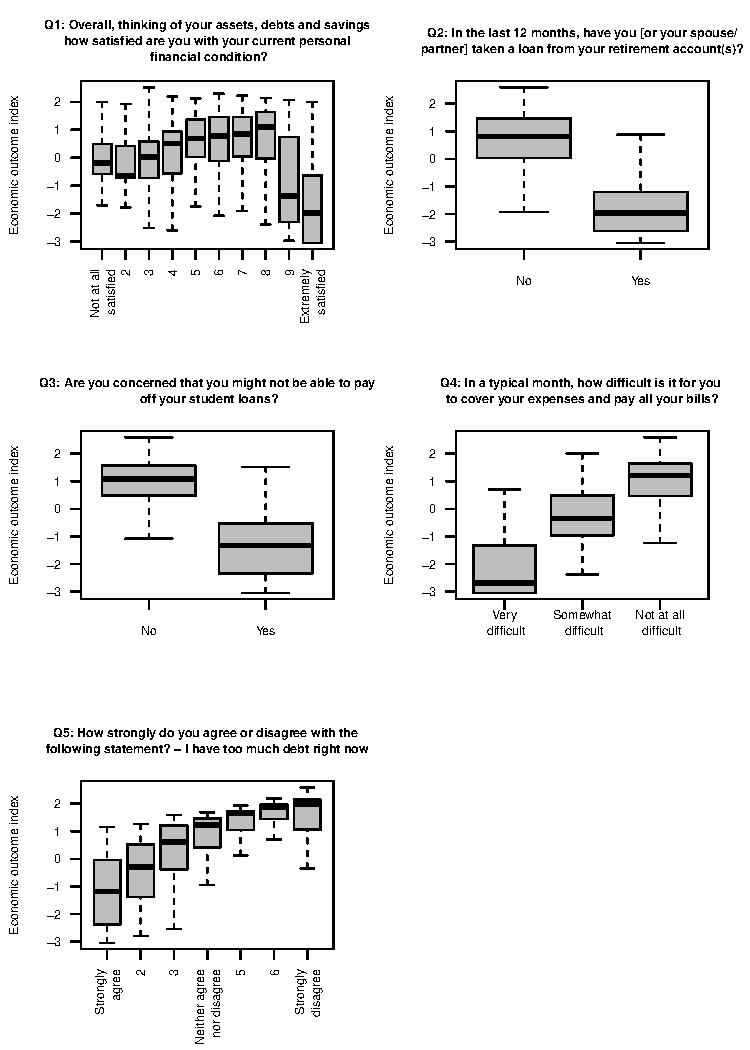
\includegraphics[scale=1.2]{biplots.pdf}}
	\label{dep1}
\end{figure}



\clearpage
\newpage 
\renewcommand{\bibsep}{0.5pt}


\begin{spacing}{1.2}
%\bibliographystyle{plain}
\bibliographystyle{apalike}
\phantomsection\addcontentsline{toc}{section}{\textbf{Bibliography}}
\bibliography{FinLit}

\end{spacing}


\end{document}

